\chapter{Felhasználói dokumentáció} % User guide
\label{ch:user}

Az alkalmazás készítése során fontos szempont volt, hogy egy felhasználóbarát webáruházat hozzak létre. A webshop használata egyszerű letisztult felülettel rendelkező program olyan funkciókkal kiegészítve, amelyik megkönnyítik az átlagos vásárlók számára az oldal kezelését. A fejezet célja, hogy bemutassa az alkalmazás azon tulajdonságait, ami nem feltétlenül egyértelmű egy hétköznapi kliens számára. Ezzel is elősegítve a webalkalmazás gördülékeny felhasználását.


\section{Alkalmazás indítása} % Enumerations and lists

Egy hétköznapi felhasználó számára talán ez a legnagyobb kihívás a program használatával kapcsolatban. Az alkalmazás indítására két módszer közül választhatunk, melyek a következőek:

\begin{compactenum}
	\item Megnyitni böngésző segítségével a weboldalt. 2.1.1. fejezet
	\item Megnyitni localhostról a projektet. 2.1.2 fejezet
\end{compactenum}

\bigskip
Mindkettő technikát részletes bemutatásra kerül a következő alfejezetekben.

\subsection{Alkalmazás indítás böngészőből}
Az első és legkönnyebben alkalmazható stratégia, hogy valamilyen előre telepített webböngésző (Chrome, Firefox, Opera..stb.) segítségével megnyitjuk az előre Amazon (AWS) szerverére telepített weboldalt. A felület ezen az url-címen érhető el: http://webbeauty.us-east-2.elasticbeanstalk.com

\subsection{Alklamazás indítása saját gépről}
Az előző  módszert azért neveztem könnyebben alkalmazhatónk, mert ha saját gépről szeretnénk indítani az alkalmazás nem csak le kell klónoznunk azt Github segítségével, hanem több különböző szoftvert kell telepítenünk mielőtt eltudnánk indítani magát a projektet. Magához a program fordításához szükségünk lesz a Node.js szoftverre, amely letölthető ingyenesen a nodejs.org eredeti honlapjáról. Továbbá még elengedhetetlen a gépünkről az Angular CLI. Ez egy parancssori interfész az Angular szoftverhez. Mivel a kód futtatásához szükségünk van rengetek eszközre, amely lefordítja és optimalizálja a kódot. A CLI ezt biztosítja a projekt számára. A kód fordításához szükségük lesz egy integrált fejlesztői környezetre. Én személy szerint a Visual Studio Code(rövidítve VS Code) nyílt forráskódú kódszerkesztőjét használtam az alkalmazás elkészítése során, így ezt fogom bemutatni. A következő felsorolásban összefoglalom azokat a lépéseket, amik segítségével eljutunk a program saját gépről való indítását. 

\begin{enumerate}
	\item\label{step:first} https://nodejs.org-ról töltsük le és telepítsük a számítógépre megfelelő .exe kiterjesztésű fájlt.
	\item https://github.com/magyardor/szakdolgozat2021 url-címen elérhető GitHub repository-t klónozzuk le az eszközünkre
	\item töltsük le, és telepítsük a Visual Studio Code nevezetű programot a https://code.visualstudio.com címről.
	\item nyissuk meg a VS code alkalmazást és installáljuk a következő bővítményeket: Angular Essentials, Material Icon Theme
	\item a VS code segítségével töltsük be a leklónozott projekt mappáját, és nyissuk meg egy új terminált
	\item a terminálba lépjünk be a szakdolgozat nevezetű mappájába és futtassuk le a következő parancssort: npm install -g @angular/cli
	\item ha ez sikeresen megtörtént akkor futtassuk le az npm i parancssort, melynek segítségével letöltődnek azok a szükséges fájlok, amik nem szerepelnek az Angular CLI interfészben, de használatban vannak 
	\item mielőtt elindítanánk az alkalmazást be kell lépnünk a projekthez tartozó MongoDB adatbázisba és hozzá kell adnunk a hálózati hozzáférés nevezetű menüpont alatt a gépünk IP címét, különben nem tud csatlakozni a szerveroldalunk az alkalmazás által megjelenítendő adatokhoz
	\item a meglévő terminálunk mellé nyissunk meg egy újat és futtassuk le az egyikbe az npm run start a másikba az npm run start:server parancsokat, az előbbi a kliensoldalt, míg az utóbbi a szerveroldali kódokat futtatja és fordítja le
	\item ha sikeresen lefordult a kód, akkor a böngésző url helyére a localhost:4200 címet begépelve megkapjuk a webáruház oldalát
\end{enumerate}


\section{Alkalmazás kezelése}
Az alkalmazás felületét két részre bonthatjuk. Az első rész maga a webáruház, amin a vásárlók megtekinthetik a termékeket és megrendelhetik őket, továbbá megnézhetik az üzemeltető által közzétett híreket, ezen felül különböző forrásokból információkat érhetnek el a vásárlással kapcsolatban. A második rész az üzemeltető által karbantartott adminisztrációs oldal. Ennek a felület használatához hitelesítés szükséges, ezzel is védve a vásárlók és a webáruház adatait. Az admin felületen lehetőség van ezen adatok kezelésére, szerkesztésére. 

\subsection{Webshop felület kezelése}
A webáruház kezelése igen egyszerű az átlagos felhasználók számára. Számos funkcióval rendelkezik az alkalmazás, amelyek elősegítik, hogy egy letisztult, felhasználóbarát programot használjanak a vásárlók.
Az áruház szerkezeti felépítése három fő részből áll:
\begin{description}
	\item[Menüsor] vagy más néven a toolbar. A \ref{fig.exemple-1}-es ábrán a webáruház főoldalának egy részét láthatjuk. A képen tetején található az alkalmazás webshopjához tartozó vezérlő felület, ami a programban toolbar néven található meg. A vezérlő felület bal oldalán látható különböző menüpontok, amelyek segítségével navigálhatunk a differens oldalak között. A jobb oldalán pedig különböző funkciókkal bíró ikonokat és az oldal logóját. Az első ilyen ikon a nyelvválasztó, aminek a segítségével megváltoztathatjuk az oldal nyelvezetét. Jelenleg az angol és a magyar nyelv közül lehet választani. A mellette lévő bevásárló kocsit ábrázoló ikon segítségével érhető el a felület kosár funkciója, ami tartalmazza az eddig hozzáadott termékeket. A kosárban szereplő termékek számáról egy előzetes információt kaphatunk a felette lévő jelvény számból.
	\begin{figure}[H]
		\centering
		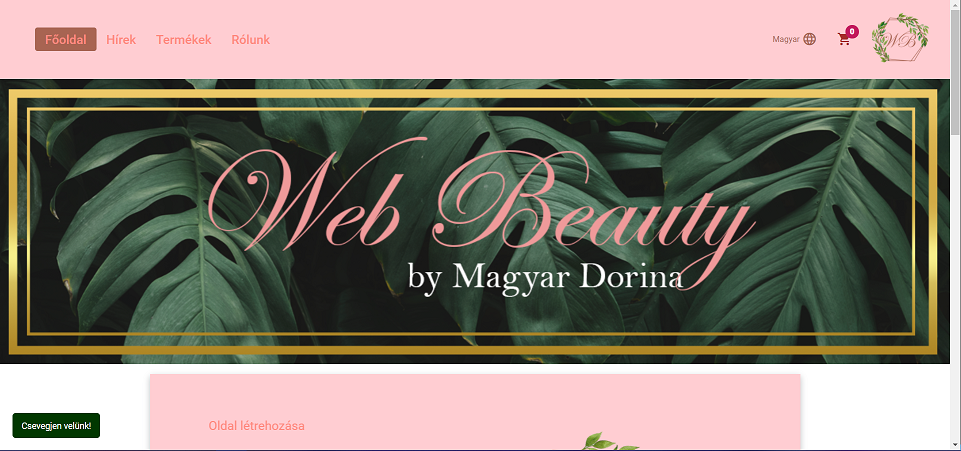
\includegraphics[width=1.0\textwidth,height=250px]{images/webshop_home.png}
		\caption{Az alkalmazás megjelenése}
		\label{fig.exemple-1}
	\end{figure}
	\item[A webáruház tartalma], amit szakmai nyelven body-nak nevezünk. Ez a menüsor alatt található meg, amit a fentebb kifejtett vezérlő felület segítségével különböző oldalak tartalmi részét jeleníthetjük meg. Példaként \ref{fig.example-2}-es ábra a és b részén láthatunk.
	\begin{figure}[H]
		\centering
		\subcaptionbox{Termékek oldala}{
			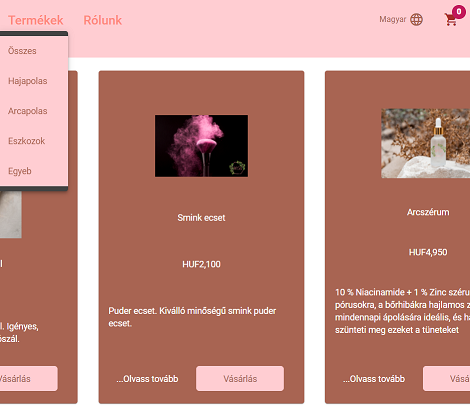
\includegraphics[width=0.45\linewidth]{images/products_page.png}}
		\hspace{5pt}
		\subcaptionbox{Hírek oldal}{
			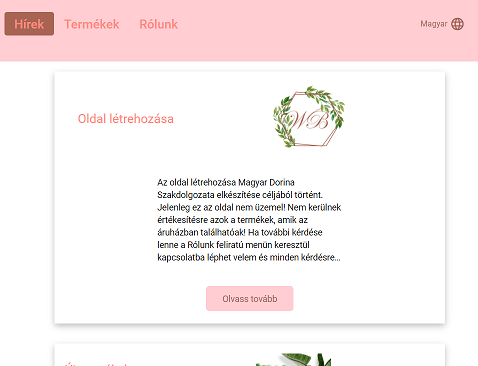
\includegraphics[width=0.45\linewidth]{images/news_page.png}}
		\caption{Webáruház tartalmi része}
		\label{fig.example-2}
	\end{figure}
	
	\item[Lábrész] vagy ahogy a programban található footer néven. A \ref{fig.exemple-3}-as képen ez a felület látható. Itt olyan oldalak linkjei jelennek meg, amik tartalmazzák a vásárlókra és az oldalra vonatkozó fogyasztóvédelmi törvényeket és általános tájékoztatókat.
	 \begin{figure}[H]
	 	\centering
	 	
\includegraphics[width=1.0\textwidth,height=120px]{images/footer.png}
	 	\caption{Az oldal lábrésze}
	 	\label{fig.exemple-3}
	 \end{figure}
	\item[Chatbot] funkció a \ref{fig.exemple-1}-es ábra legalján található zöld gomb segítségével érhető el, aminek a bemutatását a 2.3.1-es Vásárlással kapcsolatos információk alfejezetben kívánok kifejteni.
	\item[Alert üzenet] olyan információs felület, amik a felhasználó számára értesítést küld egy-egy feladat befejezésével kapcsolatban. Ilyen üzenetek lehetnek például ha nem sikerül a betöltött űrlap feldolgozása. Mint ahogy azt a \ref{fig.exemple-4}-es ábráján is láthatjuk.
	\begin{figure}[H]
		\centering
		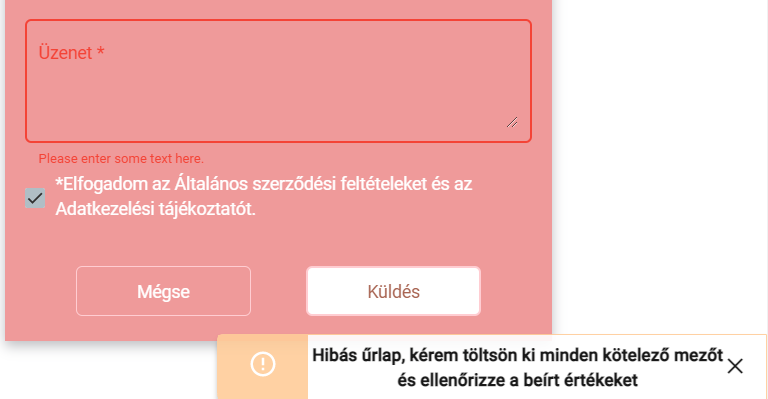
\includegraphics[width=1.0\textwidth,height=250px]{images/alert_message.png}
		\caption{Alert üzenet}
		\label{fig.exemple-4}
	\end{figure}
\end{description}


\subsection{Adminisztrációs felület kezelése} % Subfigures

In non ipsum fermentum urna feugiat rutrum a at odio. Pellentesque habitant morbi tristique senectus et netus et malesuada fames ac turpis egestas. Nulla tincidunt mattis nisl id suscipit. Sed bibendum ac felis sed volutpat. Nam pharetra nisi nec facilisis faucibus. Aenean tristique nec libero non commodo. Nulla egestas laoreet tempus. Nunc eu aliquet nulla, quis vehicula dui. Proin ac risus sodales, gravida nisi vitae, efficitur neque, Figure~\ref{fig:example-2}:

\begin{figure}[H]
	\centering
	\subcaptionbox{Vestibulum quis mattis urna}{
		\includegraphics[width=0.45\linewidth]{elte_cimer_szines}}
	\hspace{5pt}
	\subcaptionbox{Donec hendrerit quis dui sit amet venenatis}{
		\includegraphics[width=0.45\linewidth]{elte_cimer_szines}}
	\caption{Aenean porttitor mi volutpat massa gravida}
	\label{fig:example-3}
\end{figure}

Nam et nunc eget elit tincidunt sollicitudin. Quisque ligula ipsum, tempor vitae tortor ut, commodo rhoncus diam. Pellentesque habitant morbi tristique senectus et netus et malesuada fames ac turpis egestas. Phasellus vehicula quam dui, eu convallis metus porta ac.


\section{Rendelési folyamat} % Tables

Nam magna ex, euismod nec interdum sed, sagittis nec leo. Nam blandit massa bibendum mattis tristique. Phasellus tortor ligula, sodales a consectetur vitae, placerat vitae dolor. Aenean consequat in quam ac mollis. 

\begin{table}[H]
	\centering
	\begin{tabular}{ | m{0.25\textwidth} | m{0.65\textwidth} | }
		\hline
		\textbf{Phasellus tortor} & \textbf{Aenean consequat} \\
		\hline \hline
		\emph{Sed malesuada} & Aliquam aliquam velit in convallis ultrices. \\
		\hline
		\emph{Purus sagittis} &  Quisque lobortis eros vitae urna lacinia euismod. \\
		\hline
		\emph{Pellentesque} & Curabitur ac lacus pellentesque, eleifend sem ut, placerat enim. Ut auctor tempor odio ut dapibus. \\
		\hline
	\end{tabular}
	\caption{Maecenas tincidunt non justo quis accumsan}
	\label{tab:example-1}
\end{table}

\subsection{Vásárlással kapcsolatos információk} % Multi rows and multi columns

Mauris a dapibus lectus. Vestibulum commodo nibh ante, ut maximus magna eleifend vel. Integer vehicula elit non lacus lacinia, vitae porttitor dolor ultrices. Vivamus gravida faucibus efficitur. Ut non erat quis arcu vehicula lacinia. Nulla felis mauris, laoreet sed malesuada in, euismod et lacus. Aenean at finibus ipsum. Pellentesque dignissim elit sit amet lacus congue vulputate.

\begin{table}[htb]
	\centering
	\begin{tabular}{ | c | r | r | r | r | r | r | }
		\hline
		\multirow{2}{*}{\textbf{Quisque}} & \multicolumn{2}{ c | }{\textbf{Suspendisse}} & \multicolumn{2}{ c | }{\textbf{Aliquam}} & \multicolumn{2}{ c | }{\textbf{Vivamus}} \\
		\cline{2-7}
		& Proin & Nunc & Proin & Nunc & Proin & Nunc \\
		\hline \hline		
		Leo & 2,80 MB & 100\% & 232 KB & 8,09\% & 248 KB & 8,64\% \\
		\hline
		Vel & 9,60 MB & 100\% & 564 KB & 5,74\% & 292 KB & 2,97\% \\
		\hline
		Auge & 78,2 MB & 100\% & 52,3 MB & 66,88\% & 3,22 MB & 4,12\% \\
		\hline 
	\end{tabular}
	\caption[Rövid cím a táblázatjegyzékbe]{Vivamus ac arcu fringilla, fermentum neque sed, interdum erat. Mauris bibendum mauris vitae enim mollis, et eleifend turpis aliquet.}
	\label{tab:example-2}
\end{table}

\subsection{Rendelés leadása} % Long tables over multiple pages

Nunc porta placerat leo, sit amet porttitor dui porta molestie. Aliquam at fermentum mi. Maecenas vitae lorem at leo tincidunt volutpat at nec tortor. Vivamus semper lacus eu diam laoreet congue. Vivamus in ipsum risus. Nulla ullamcorper finibus mauris non aliquet. Vivamus elementum rhoncus ex ut porttitor.